\begin{figure}
\centering
\begin{minipage}{.45\textwidth}
  \centering
	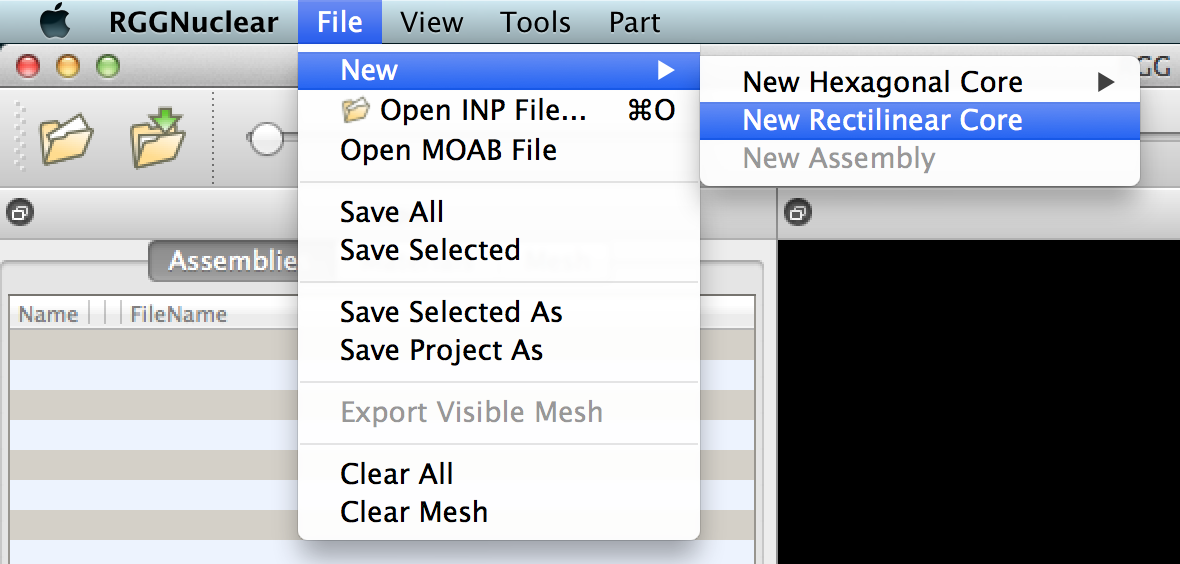
\includegraphics[width=0.9\linewidth]{Images/rect-1e1.png}
	\caption{Select the option to create a new rectilinear assembly duct.}
	\label{fig:Rect1}
\end{minipage} \hspace{.5cm}%
\begin{minipage}{.45\textwidth}
  \centering
	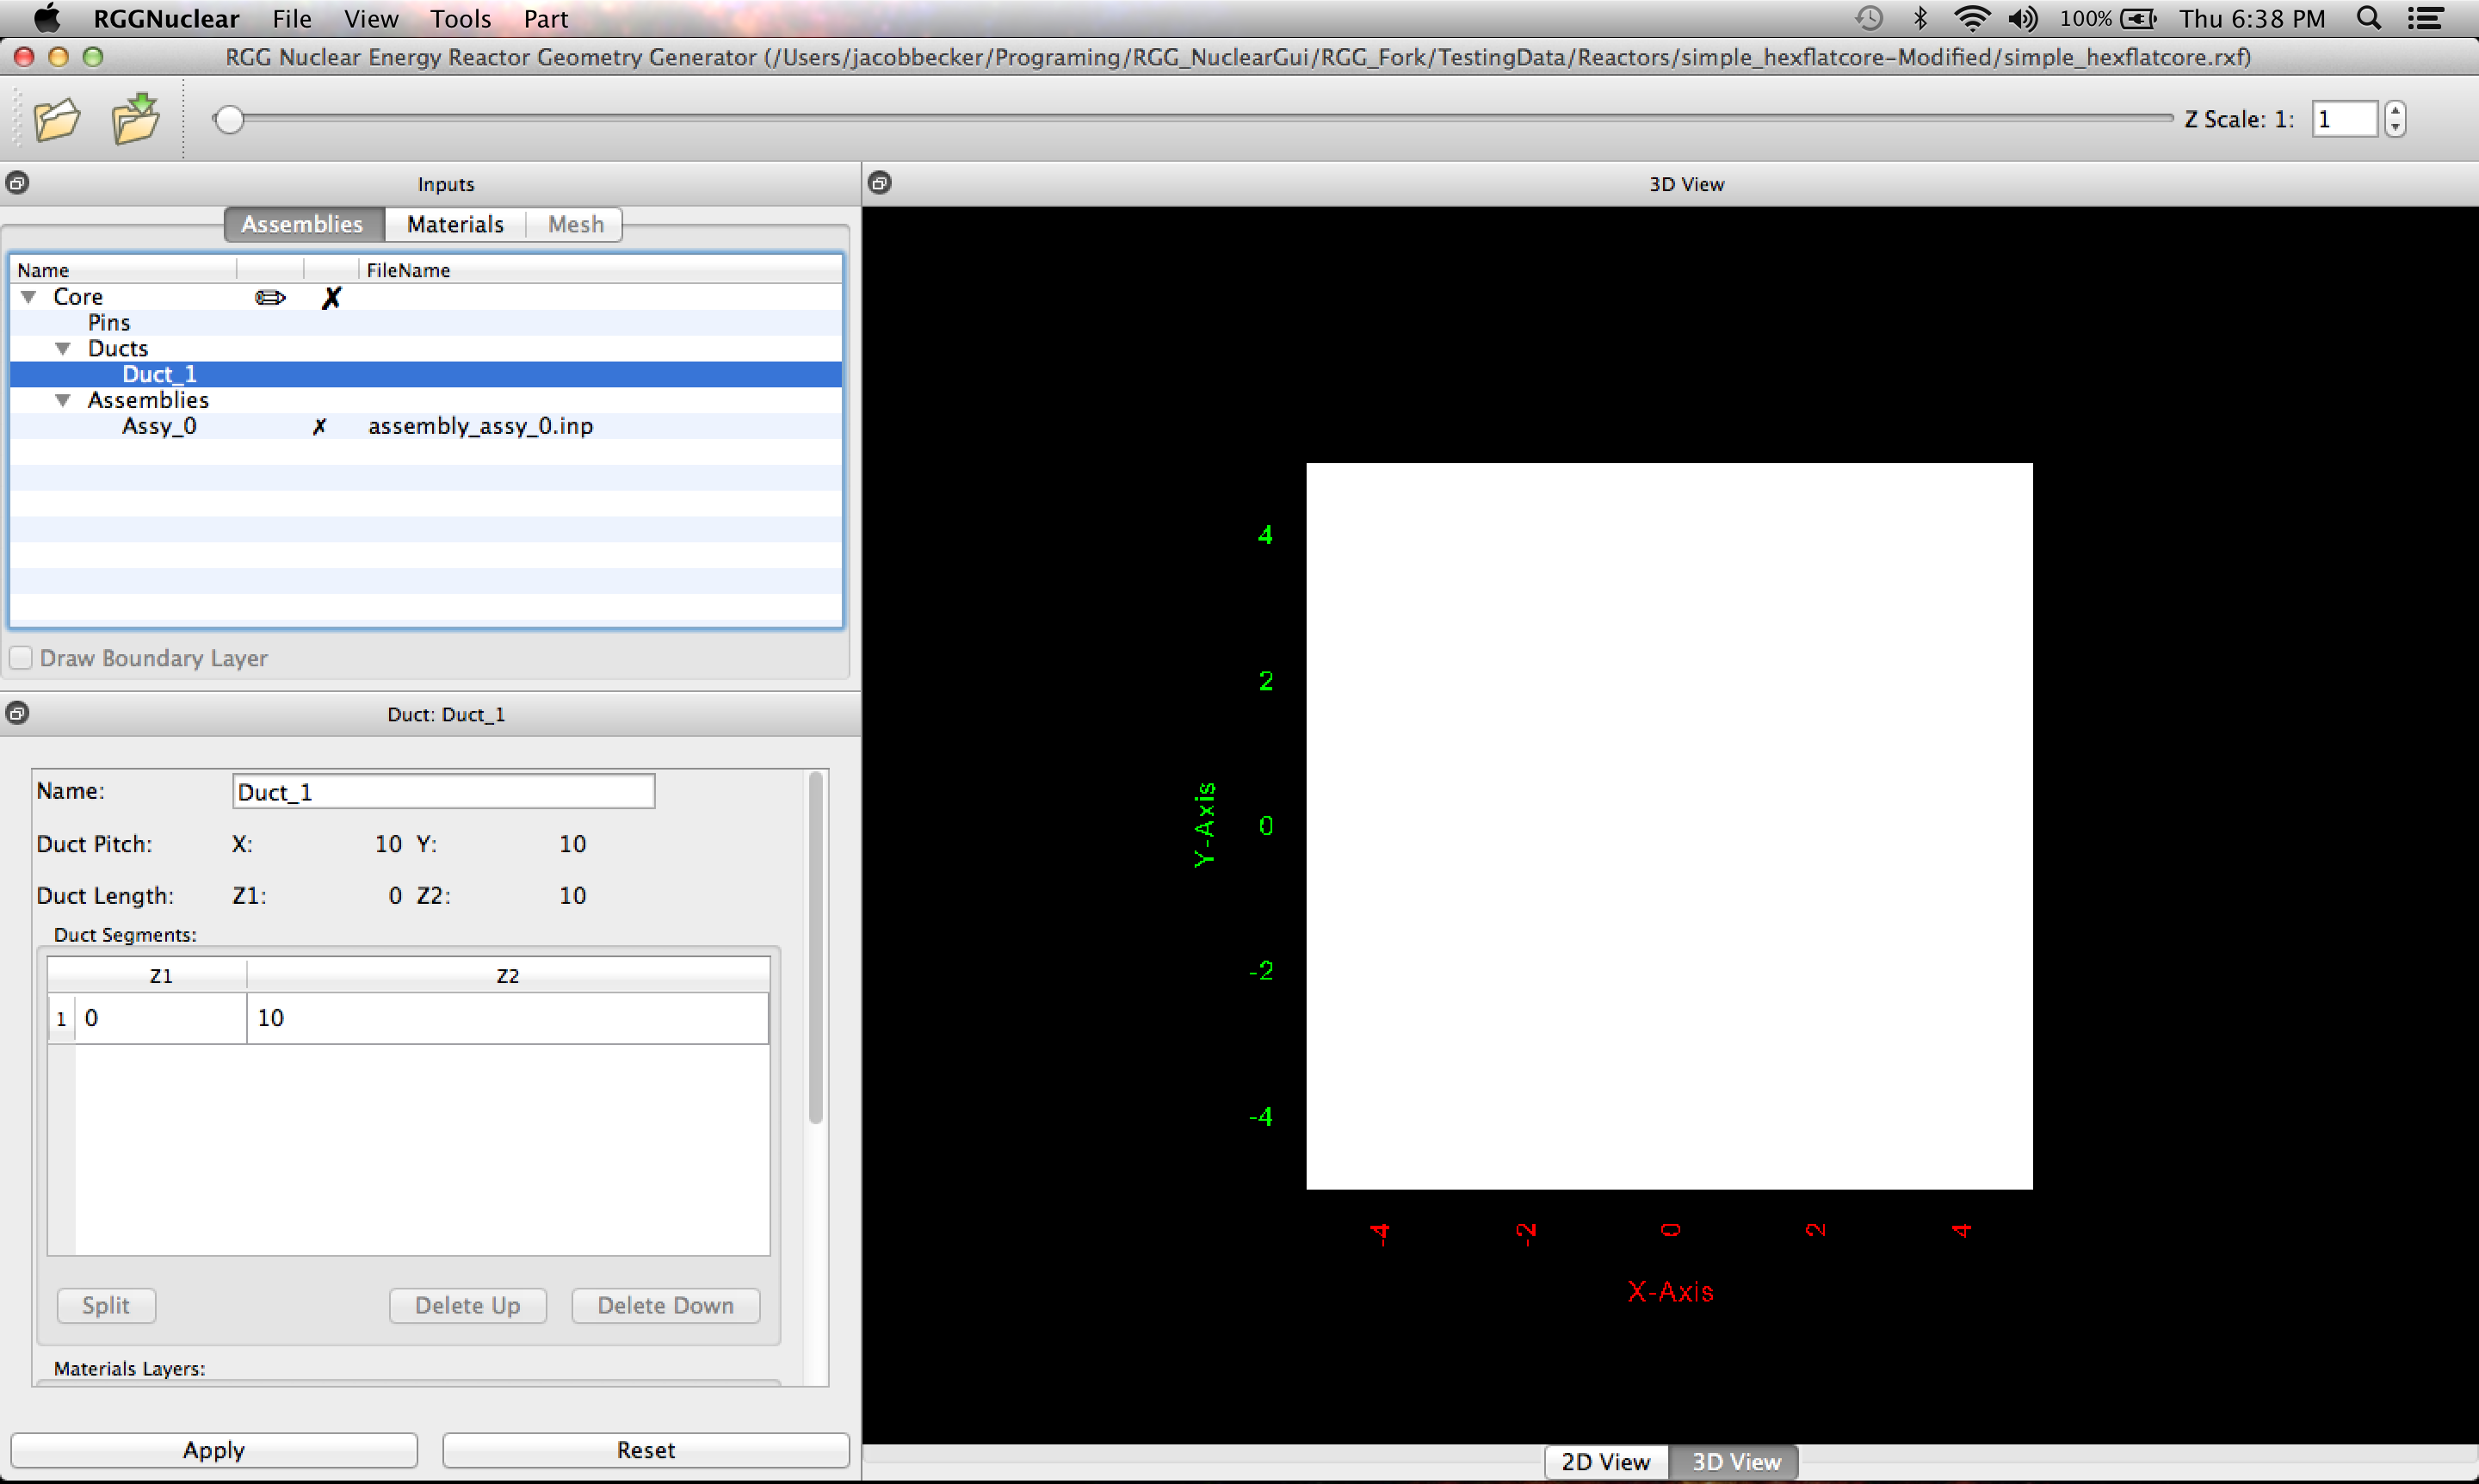
\includegraphics[width=0.9\linewidth]{Images/rect-init-model.png}
	\caption{The initial rectangular core.}
	\label{fig:NewRect}
\end{minipage}
\end{figure}

\begin{wrapfigure}{R}{0.5\textwidth}
\vspace{-60pt}
  \begin{center}
    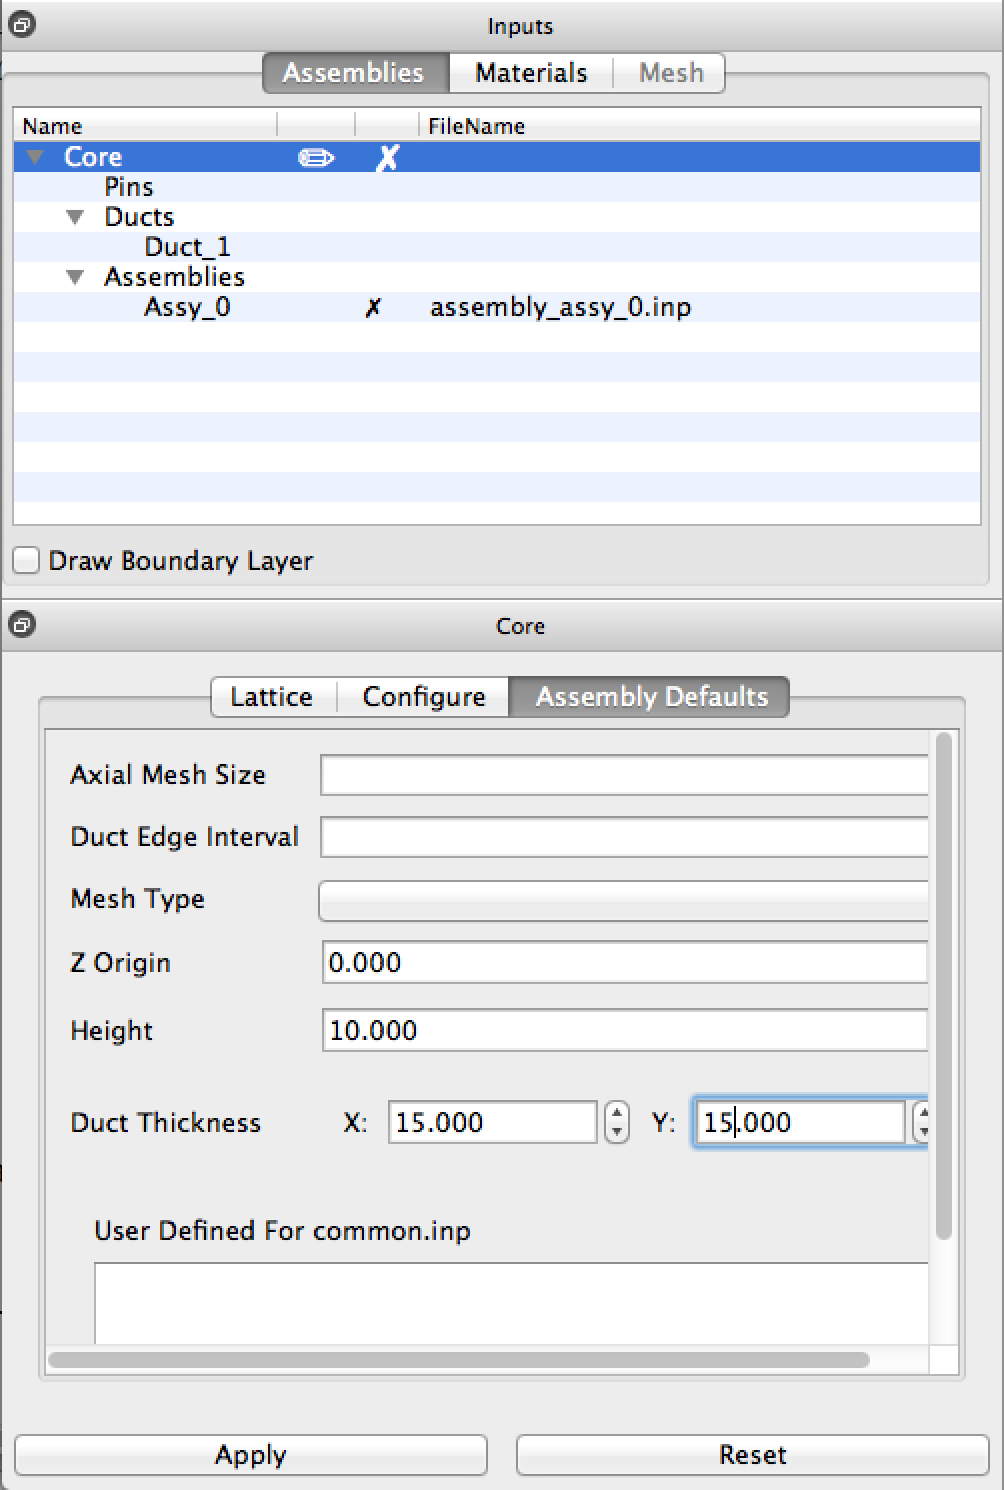
\includegraphics[width=0.75\linewidth]{Images/rect-set-dim.png}
  \end{center}
 \caption{Setting the global duct parameters.}
\label{fig:SetRectDuctDem}
\vspace{-60pt}
\end{wrapfigure}

\subsection{Creating an Assembly Duct}

First, create a new rectilinear core, and add a new duct to the assembly by following Figure \ref{fig:Rect1}.

This results in a core with a single assembly with a duct of unknown material shown in Figure \ref{fig:NewRect}.

Now, to adjust the size of the duct, select the "\ui{Assembly Defaults}" tab in Core's Properties Panel.  In this example, we are going to set the ``\ui{Duct Thickness}[Assembly Defaults]" to 15 (Figure\ref{fig:SetRectDuctDem}).

Next adjust the material of the \ui{Duct}.  In the \ui{Inputs Panel}, select the \ui{Duct}, in this case Duct\_1.  Then, in the Duct's \ui{Properties Panel}[Duct], select the first Duct Segment.  This populates Material Layers with the Duct Segments materials.  Now, select water in the material drop down box drop (Figure \ref{fig:rectSetMaterial}).  Then press Apply.  The result should look like Figure \ref{fig:rectDuctResult}.

\begin{figure}[hb]
\centering
\begin{subfigure}{.4\textwidth}
  \centering
  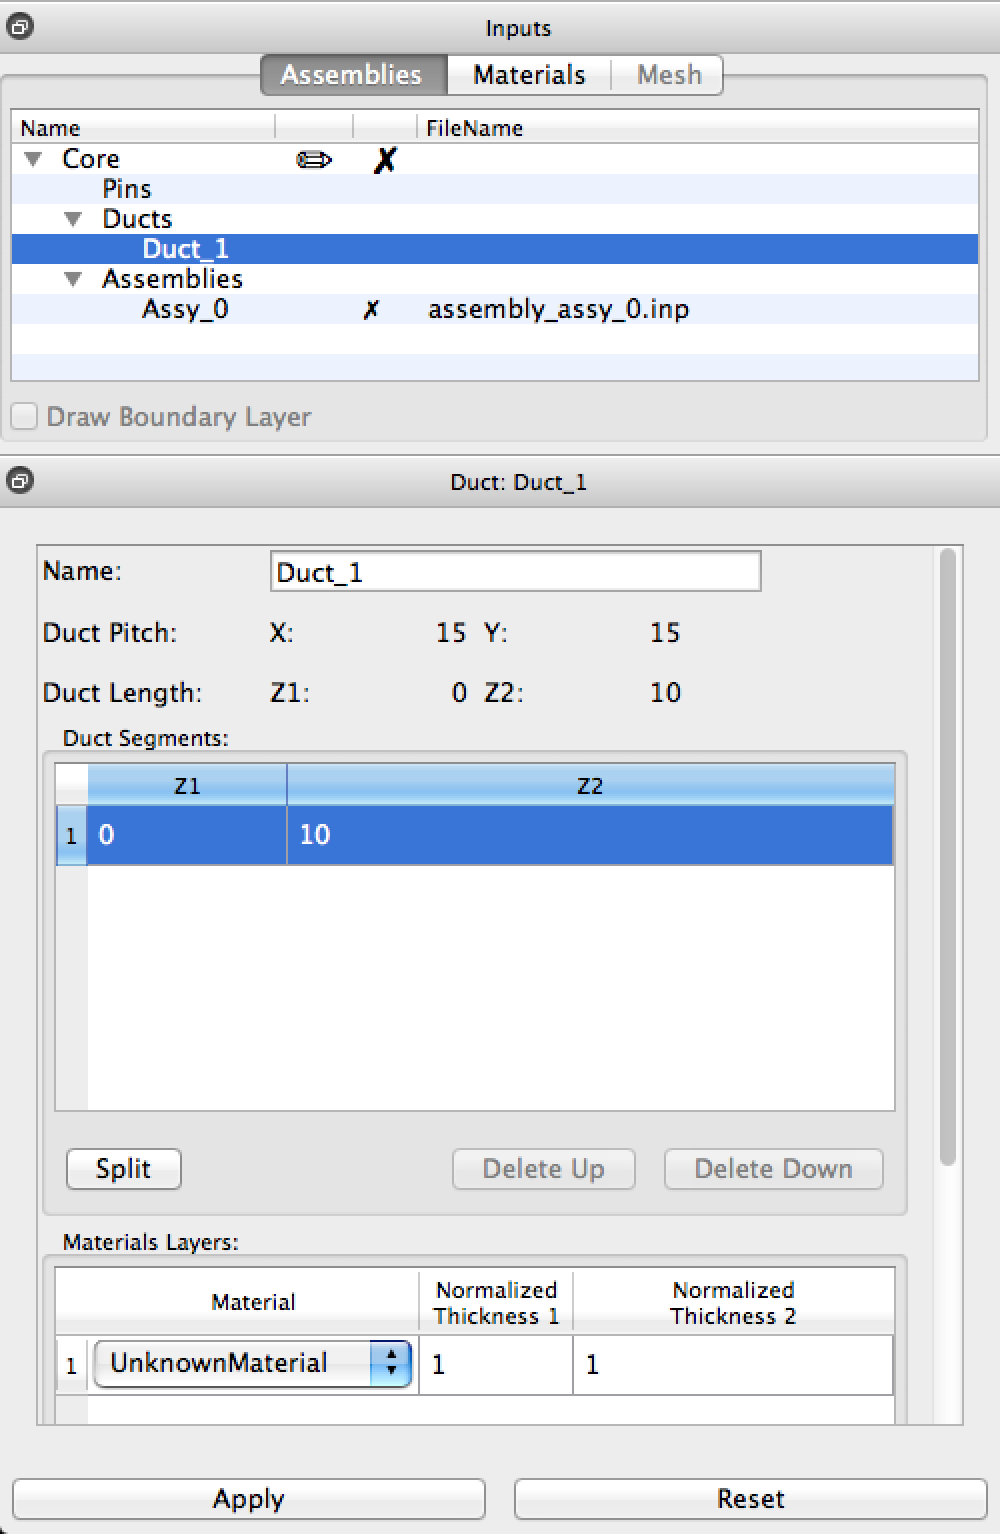
\includegraphics[width=0.5\linewidth]{Images/rect-set-material.png}
  \caption{Setting material of the duct.}
  \label{fig:rectSetMaterial}
\end{subfigure}%
\begin{subfigure}{.6\textwidth}
  \centering
  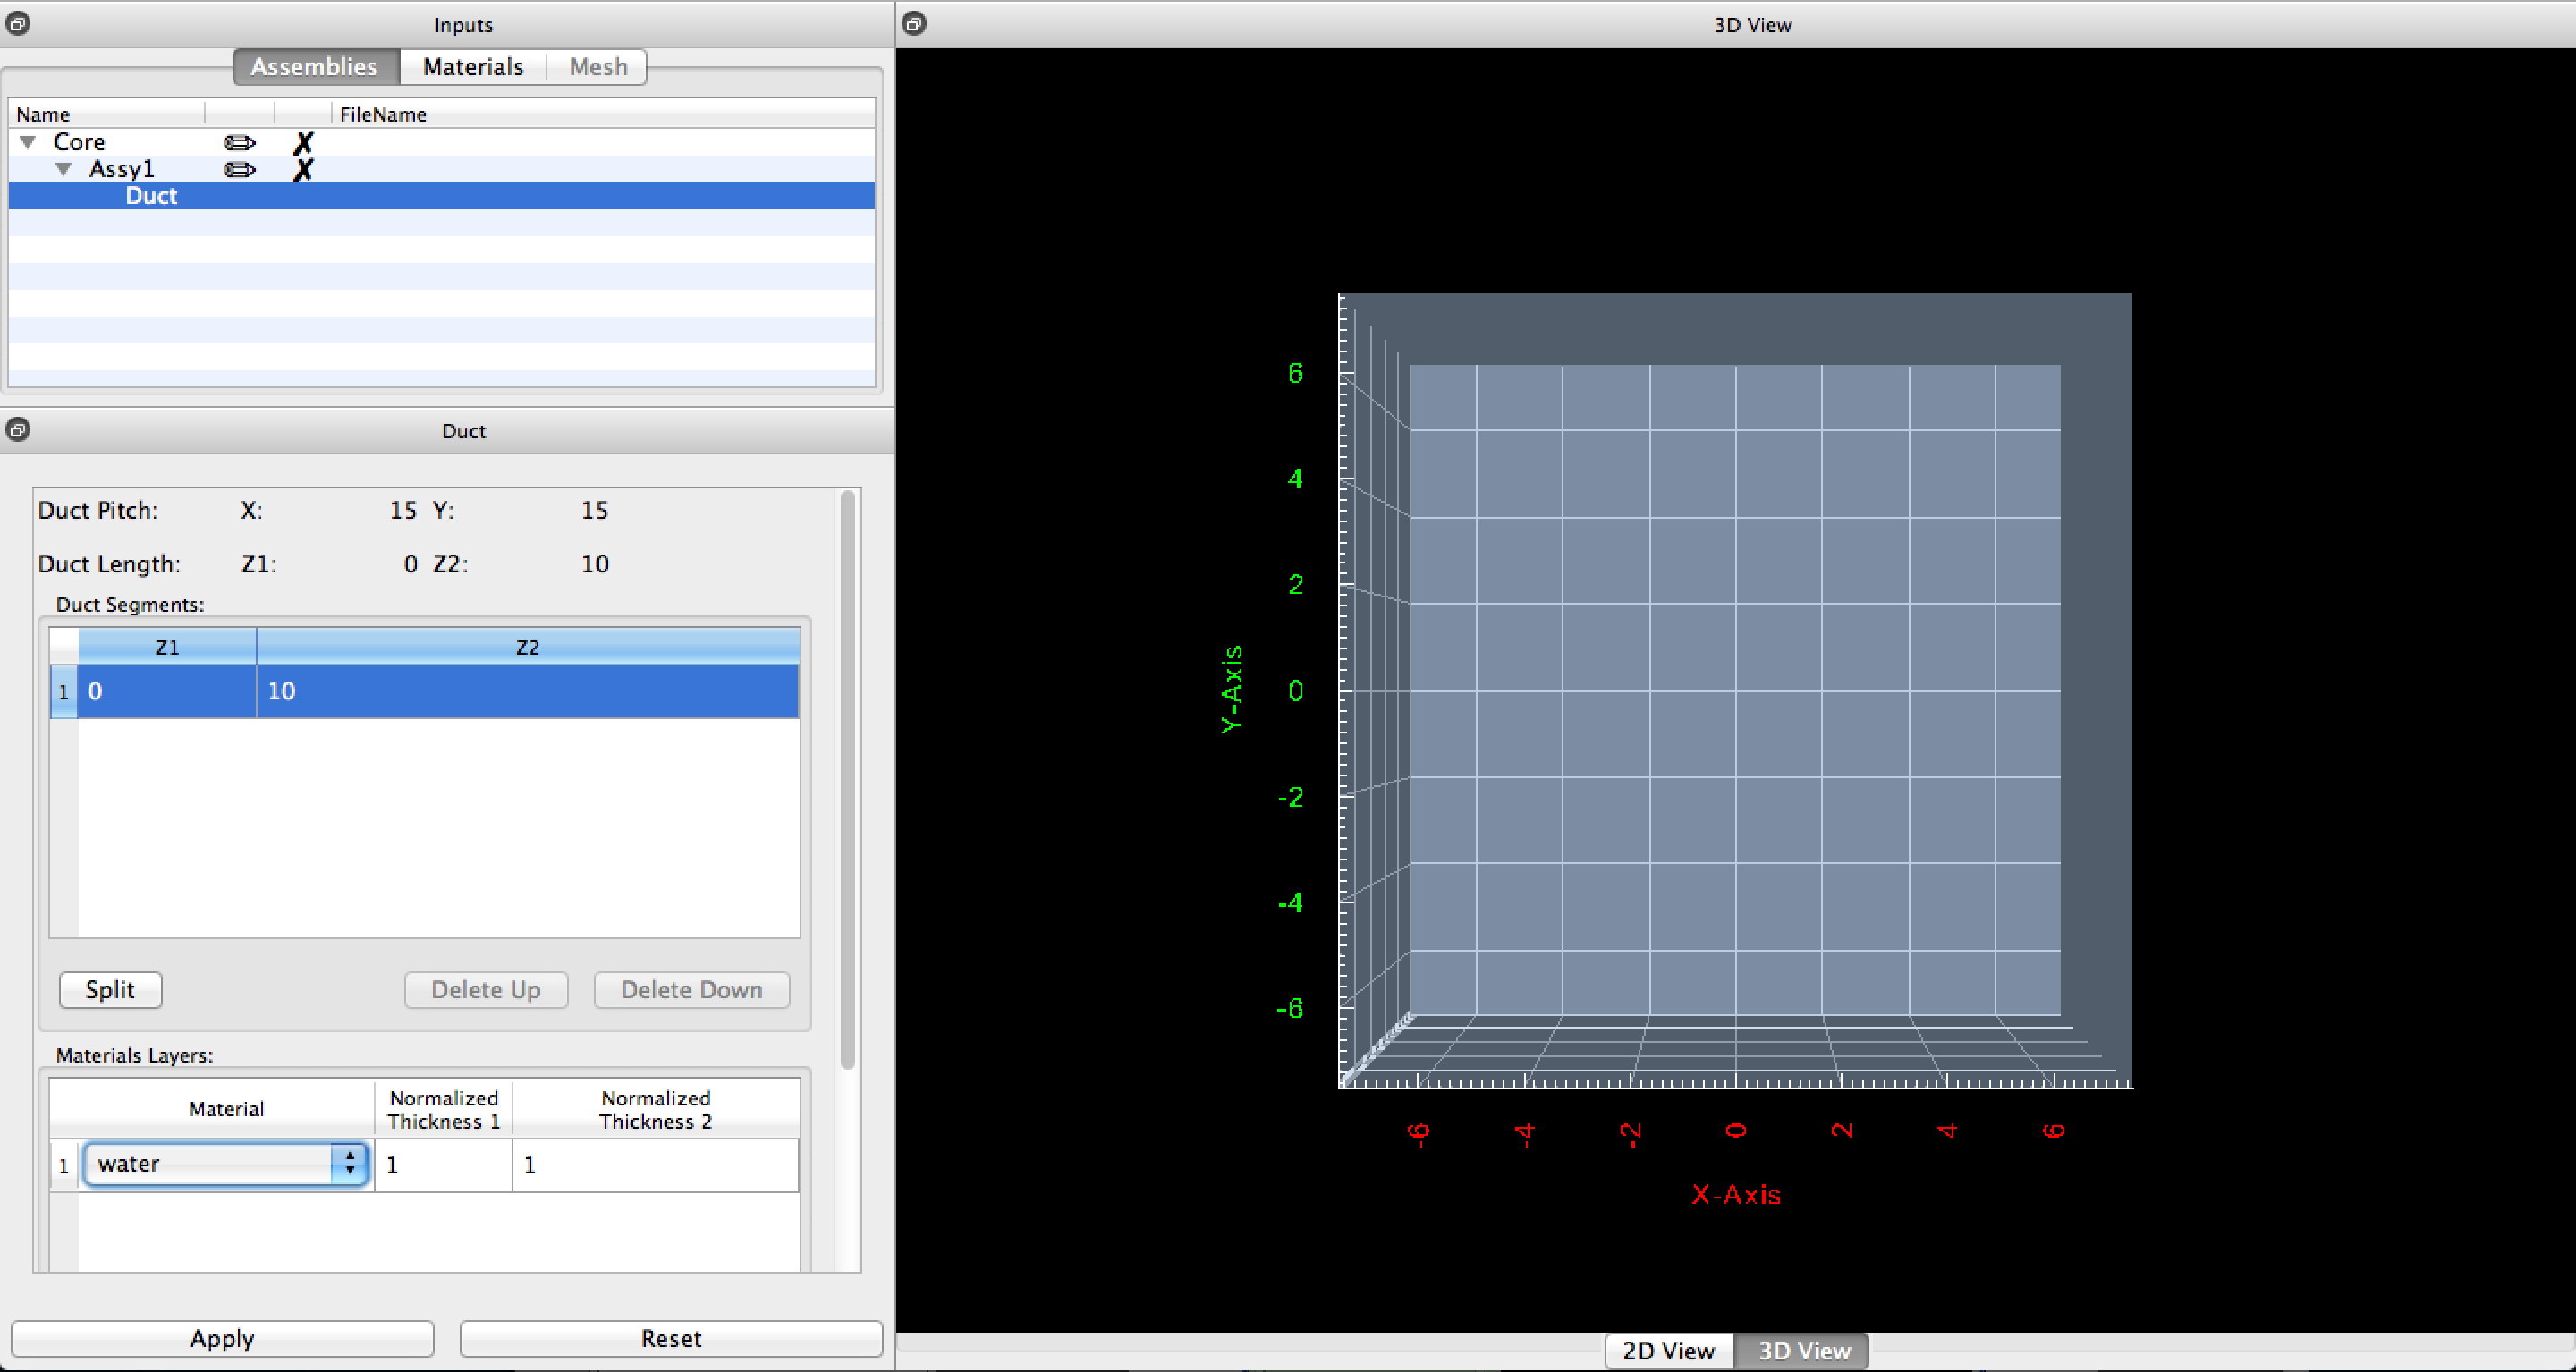
\includegraphics[width=0.9\linewidth]{Images/rect-duct-result.png}
  \caption{The final product.}
  \label{fig:rectDuctResult}
\end{subfigure}
\caption{Finished water duct.}
\label{fig:test}
\end{figure}

\begin{commonerrors}
	When finishing editing properties, make sure to hit 
	apply before switch to another component in the Assemblies tab.
\end{commonerrors}


\subsection{Creating a Fuel Pin}

Right-click on the assembly and choose ``Create Pin'' (Figure \ref{fig:rectCreatePin}).

\begin{figure}
\centering
\begin{minipage}{.4\textwidth}
       \begin{center}
	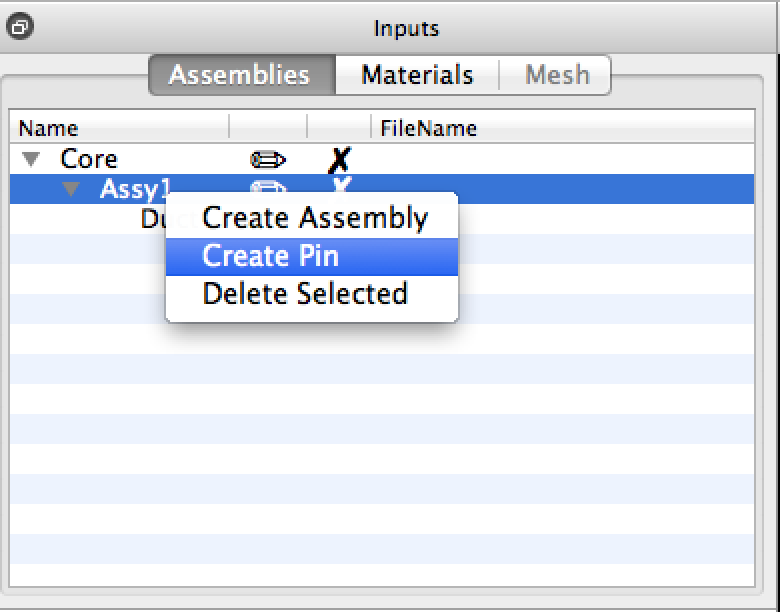
\includegraphics[width=0.70\linewidth]{Images/rect-create-pin-option.png}
	\caption{Create pin option.}
	\label{fig:rectCreatePin}
     \end{center}
\vspace{15pt}
     \begin{center}
	 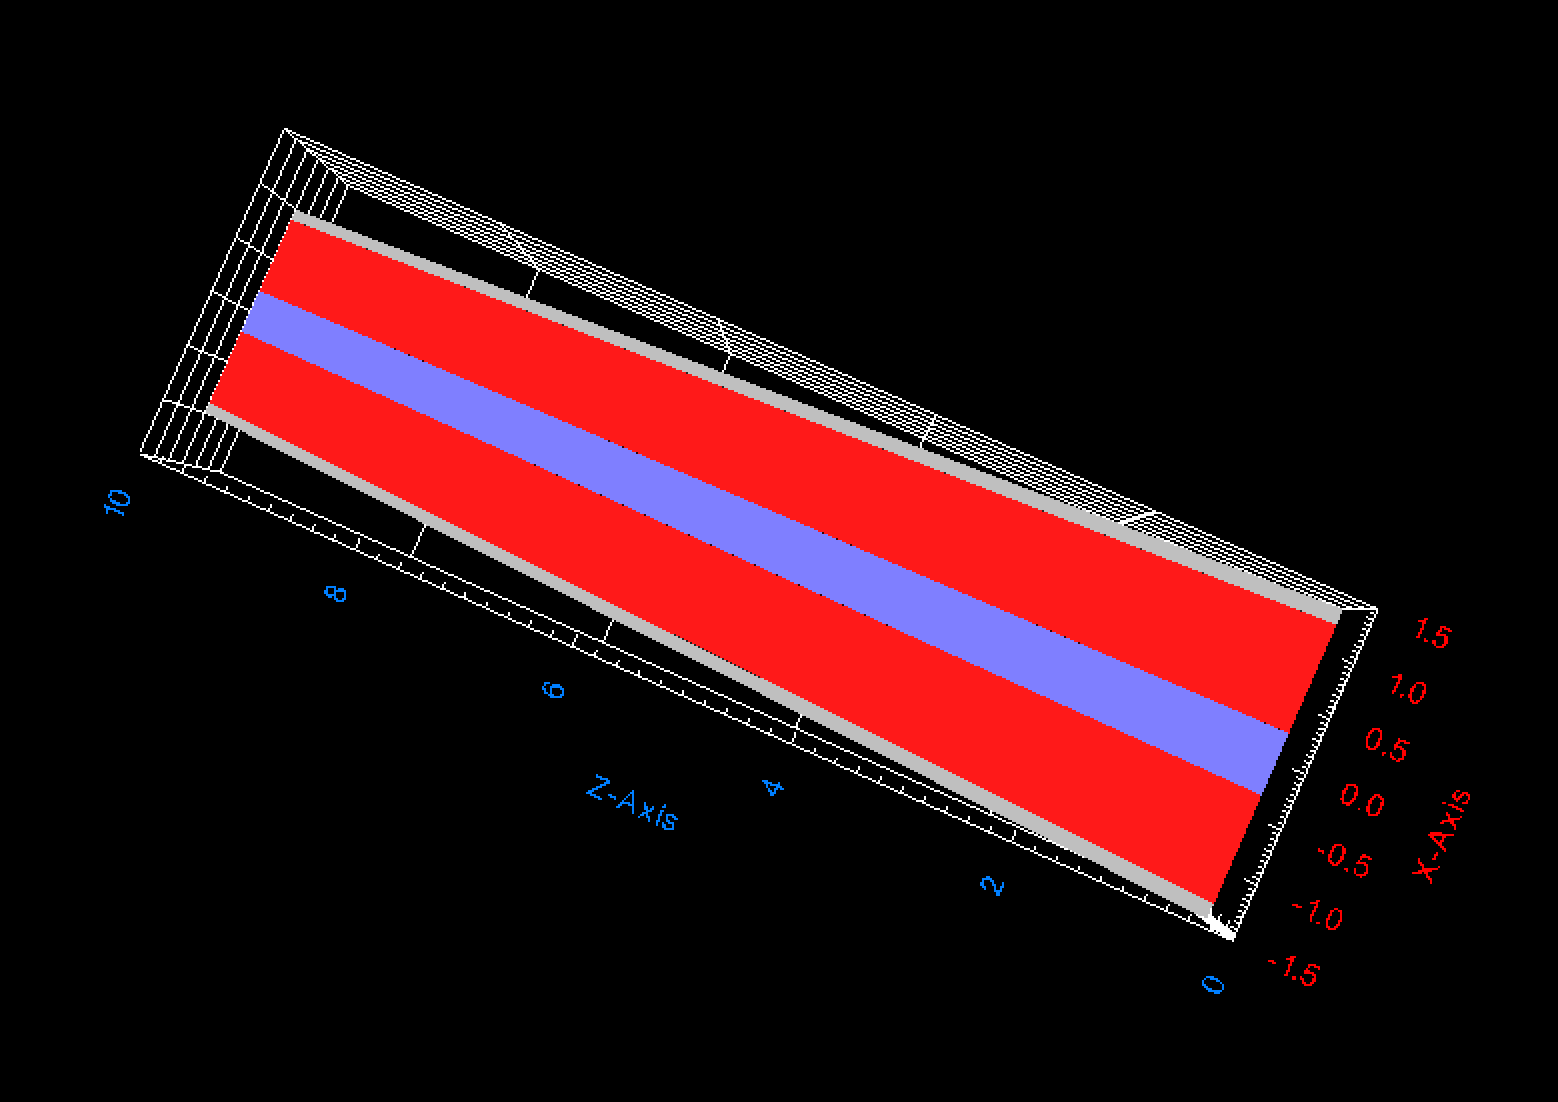
\includegraphics[width=0.70\textwidth]{Images/rect-pin.png}
	 \caption{Final fuel pin product.}
  	\label{fig:Rect6}
      \end{center}
\end{minipage} \hspace{.5cm}%
\begin{minipage}{.4\textwidth}
  \centering
	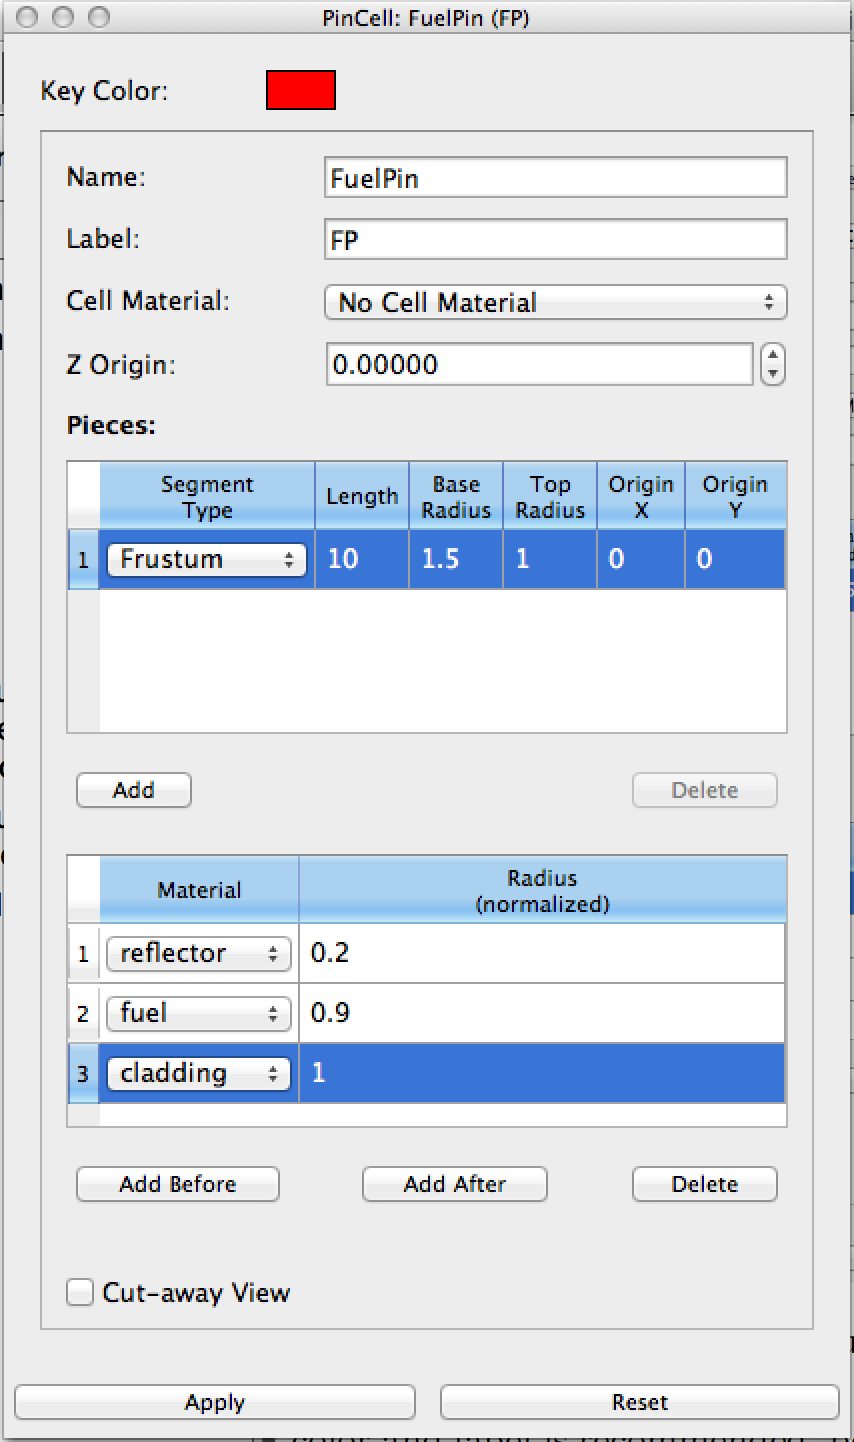
\includegraphics[width=0.65\linewidth]{Images/rect-pin-params.png}
	\caption{Fuel pin parameters.}
	\label{fig:Rect5}
\end{minipage}
\end{figure}

\subsubsection{Changing the Parameters}

Choose the dimensions of the pin to correspond to the dimensions of your duct.  In our case we have used a length of 10, corresponding to the height of the duct.


Changing the key color and label is recommended, because later this will make the fuel pin more recognizable while organizing the assembly.


Using the ``Add Before'' button, you can create a fuel pin with different layers of materials.  Refer to Figure \ref{fig:Rect5} for the parameters used for our example, and Figure \ref{fig:Rect6} to view the final product.

Note also the option to toggle the fuel pin's shape between a cylinder and a frustum.  The ``\ui{Cutaway view}'' helps to view how the different materials are distributed within the fuel pin.

Control rods are used to control nuclear fission. They are made out of materials which can easily absorb neutrons without undergoing fission themselves such as certain isotopes of boron, silver, or cadmium.

This is created using largely the same process as creating the fuel pin.  You can use the ``control rod'' material.  Once again, it's beneficial to change the key color to green.

Refer to Figure \ref{fig:Rect7} for the final product.

\subsection{Adding Fuel Pins to the Assembly}

\begin{wrapfigure}{R}{0.6\textwidth}
  \vspace{-10pt}
  \begin{center}
    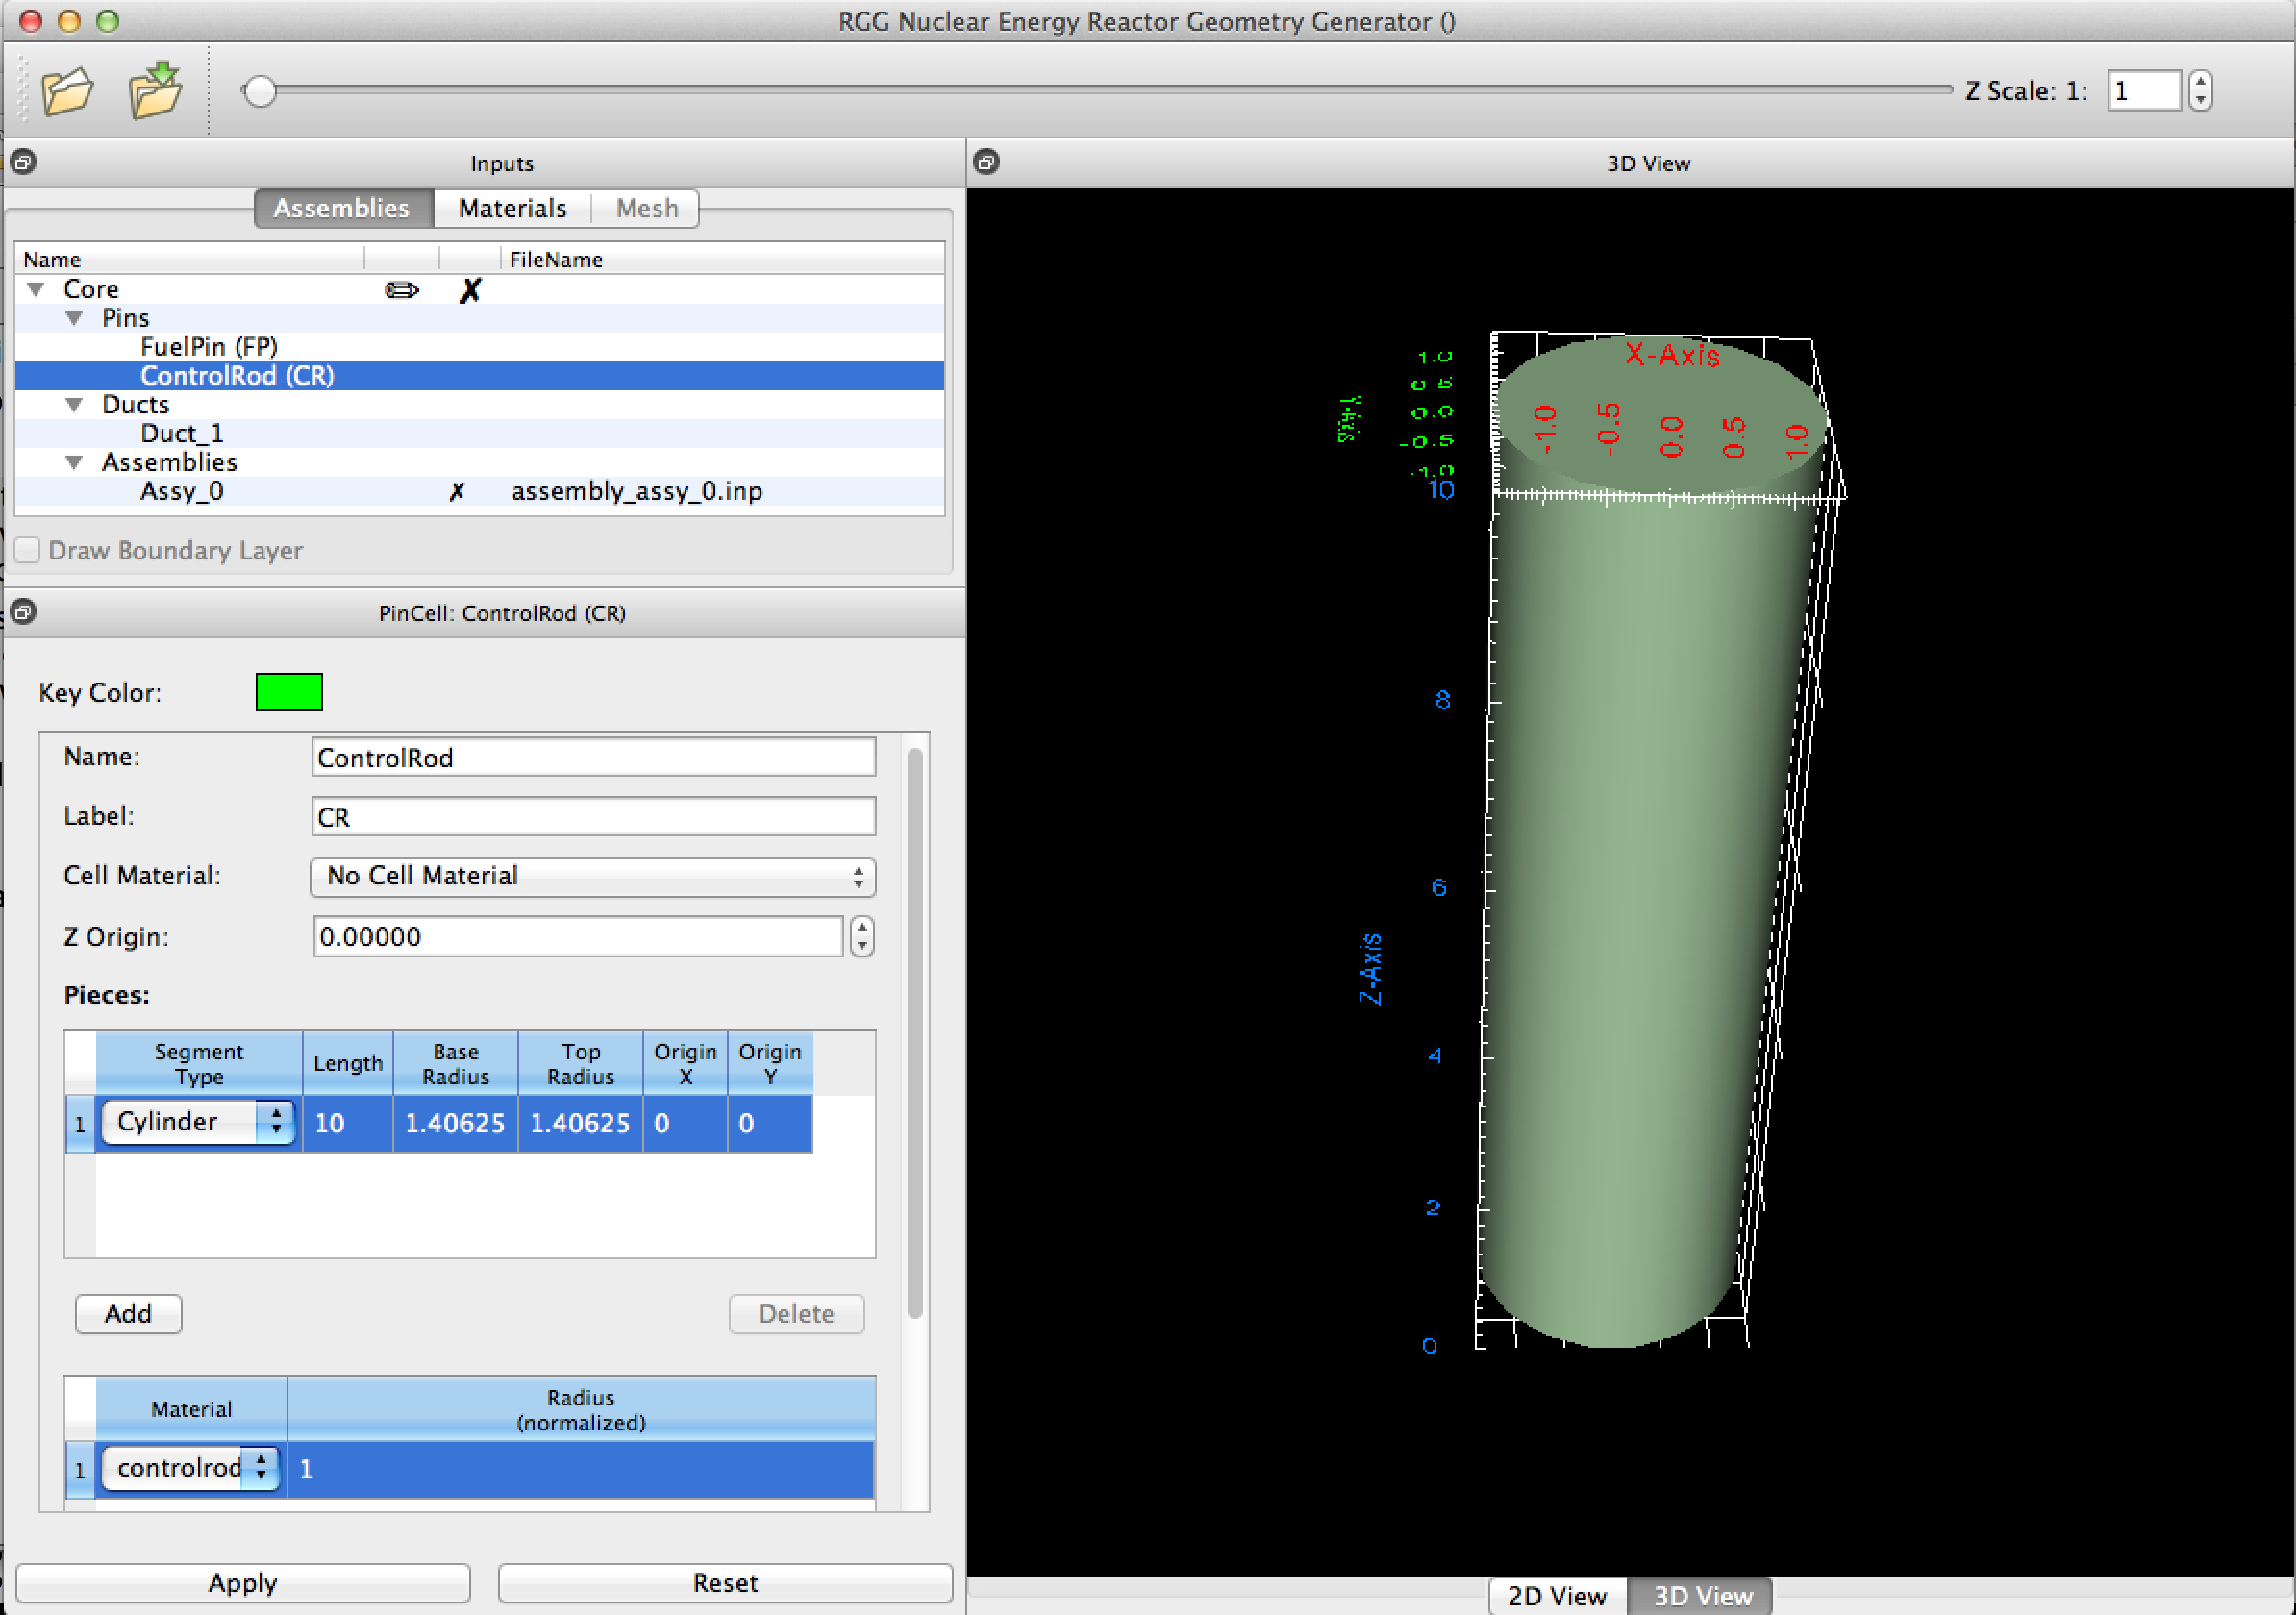
\includegraphics[width=0.8\linewidth]{Images/rect-control-rod.png}
  \end{center}
  \caption{Final control product.}
  \label{fig:Rect7}
  \vspace{-20pt}
\end{wrapfigure}

\begin{figure}[H]
\centering
\begin{minipage}{.5\textwidth}
  \centering
  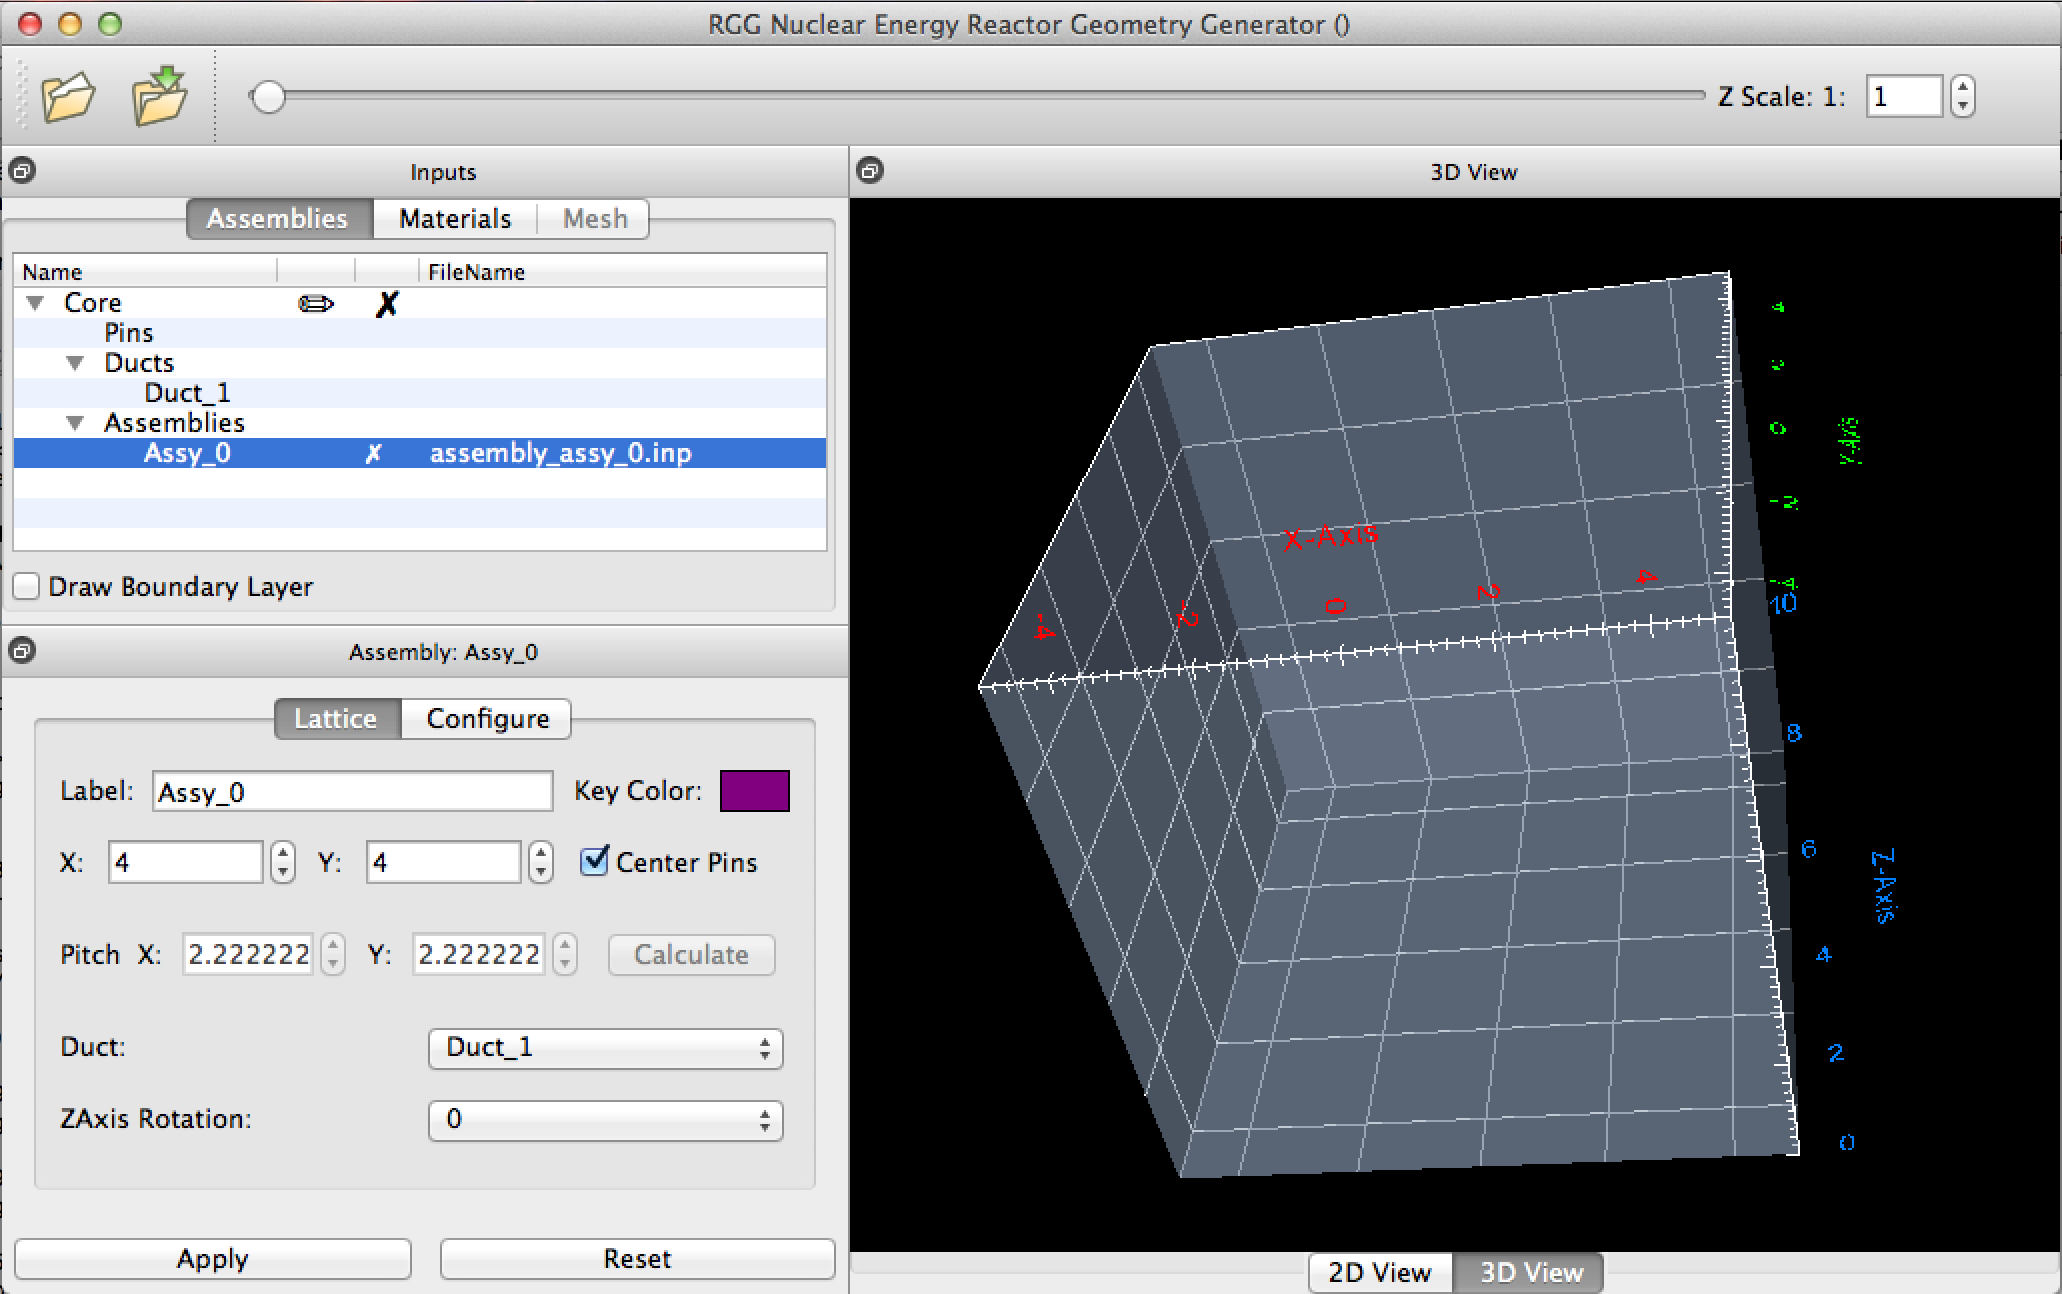
\includegraphics[width=0.90\linewidth]{Images/rect-empty-assy.png}
\caption{Empty duct in the assemblies view.}
\label{fig:Rect8}
\end{minipage}%
\hspace{0.5cm}
\begin{minipage}{.35\textwidth}
  \centering
 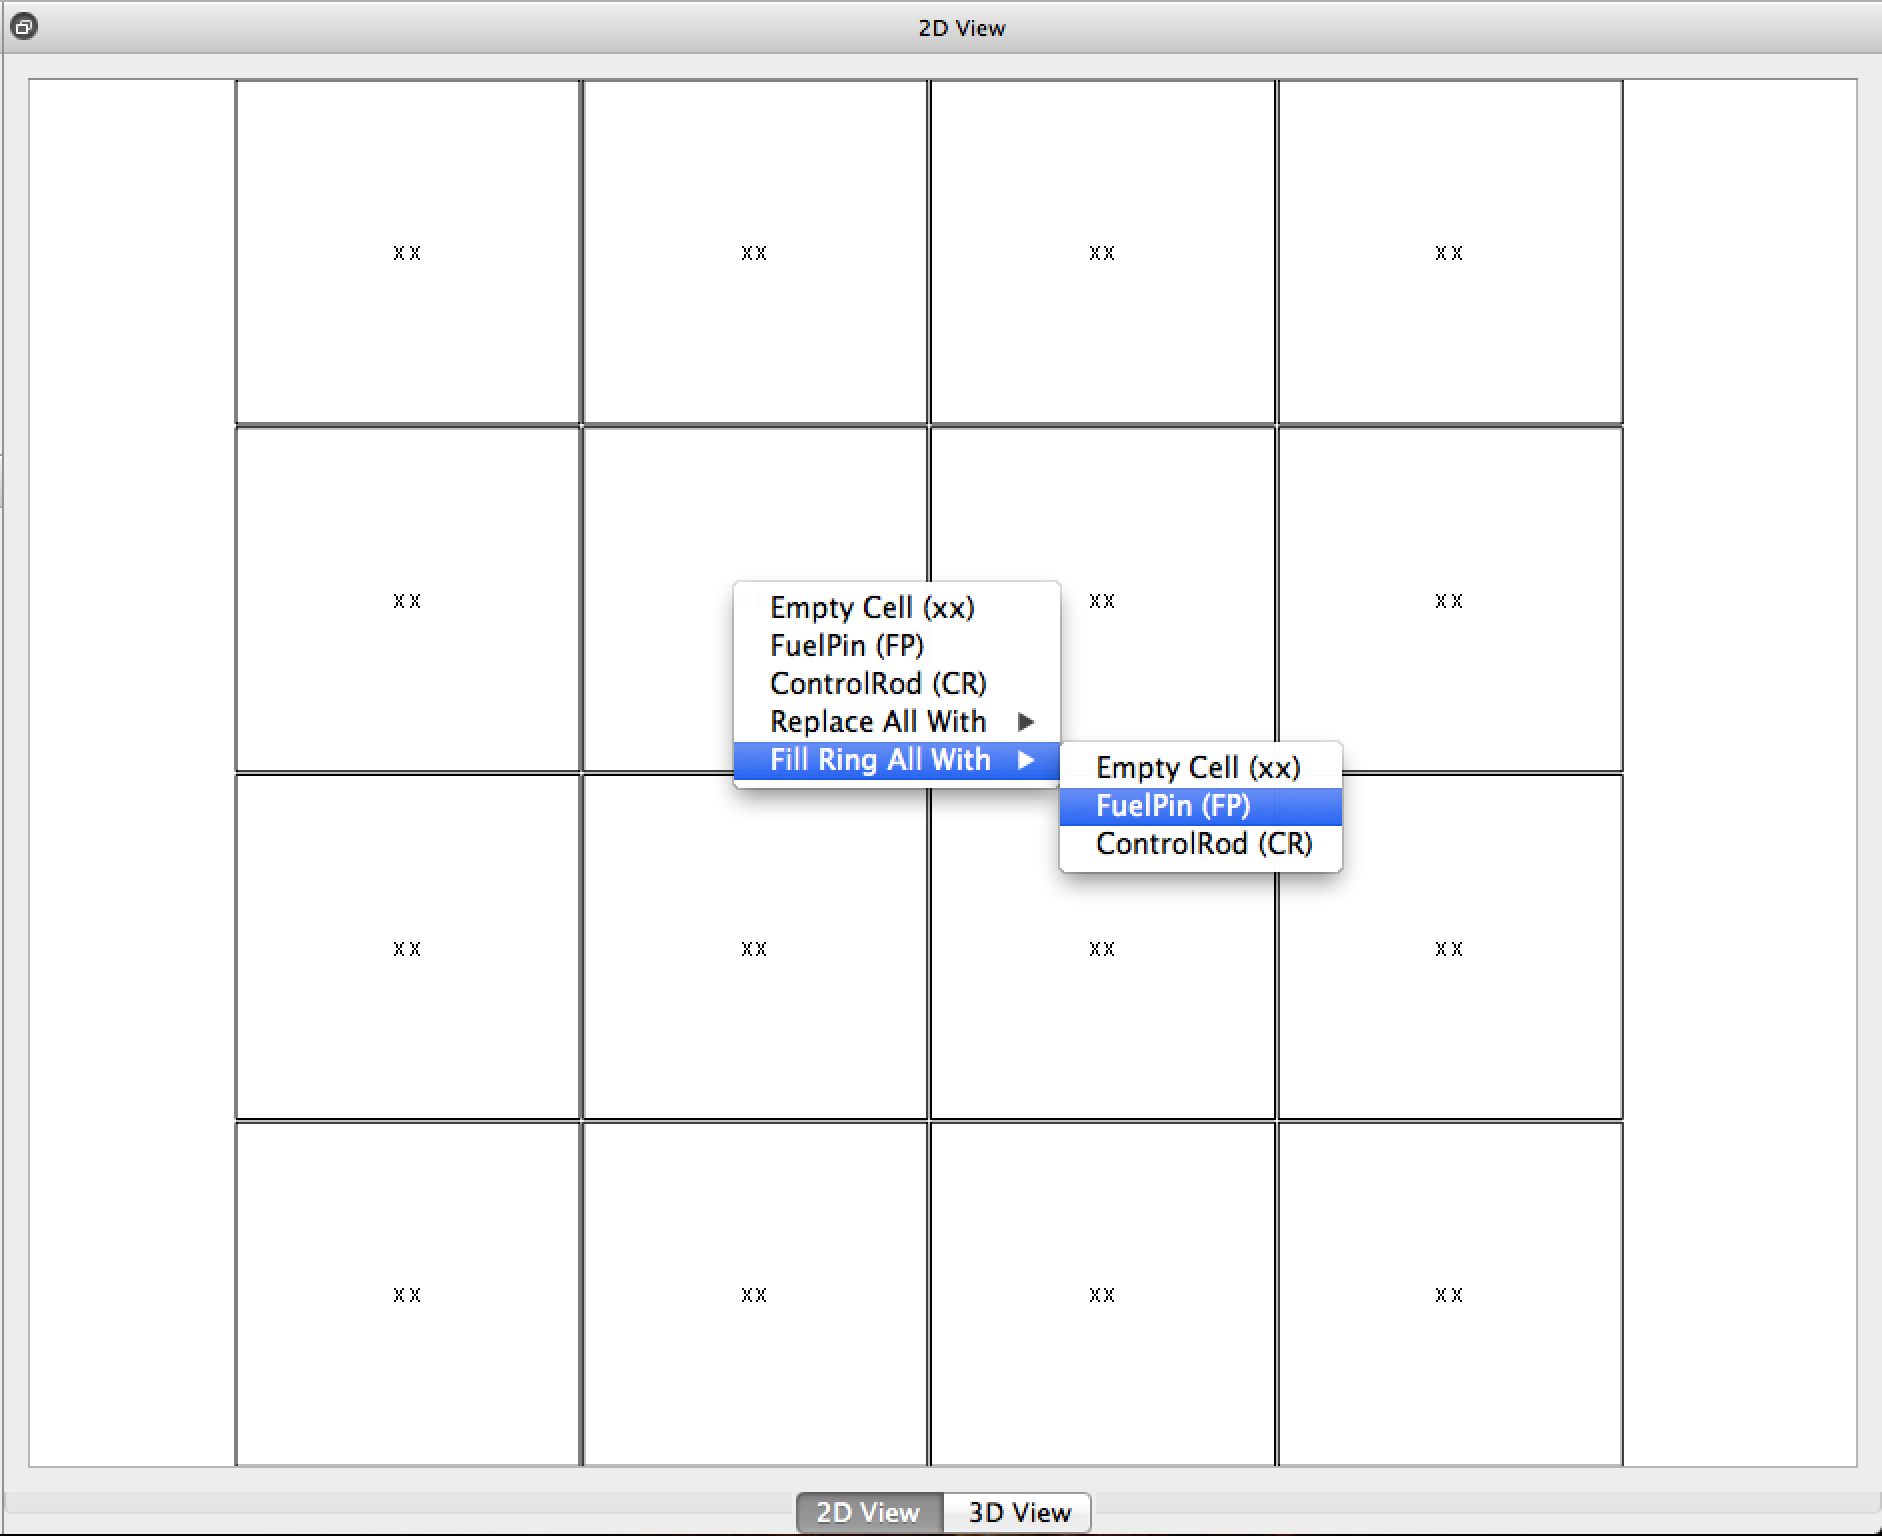
\includegraphics[width=0.9\linewidth]{Images/rect-assign-pin.png}
\caption{Right-click to organize the assembly.}
\label{fig:Rect9}
\end{minipage}
\end{figure}

Now we want to add the pins we've created back to the assembly.  Click back on ``Assy\_0'' in the assemblies view in order to see the assembly layout.  You should once again be able to see the water duct you created, and it should still be empty.  Compare your view with Figure \ref{fig:Rect8}.

Right click on each square and choose which pin to assign to it.  For the fuel rod, we want it to fill the center ring, so we select fuel in \ui{Fill Ring With}.  Alternatively, you can drag and drop pins already placed onto new squares.

In the end you should end up with something like ~\ref{fig:Rect10}.

Remember to click ``Apply'' in order to see your changes in the render window, or save them before navigating to another tab or pin.

\begin{figure}[h]
\begin{center}
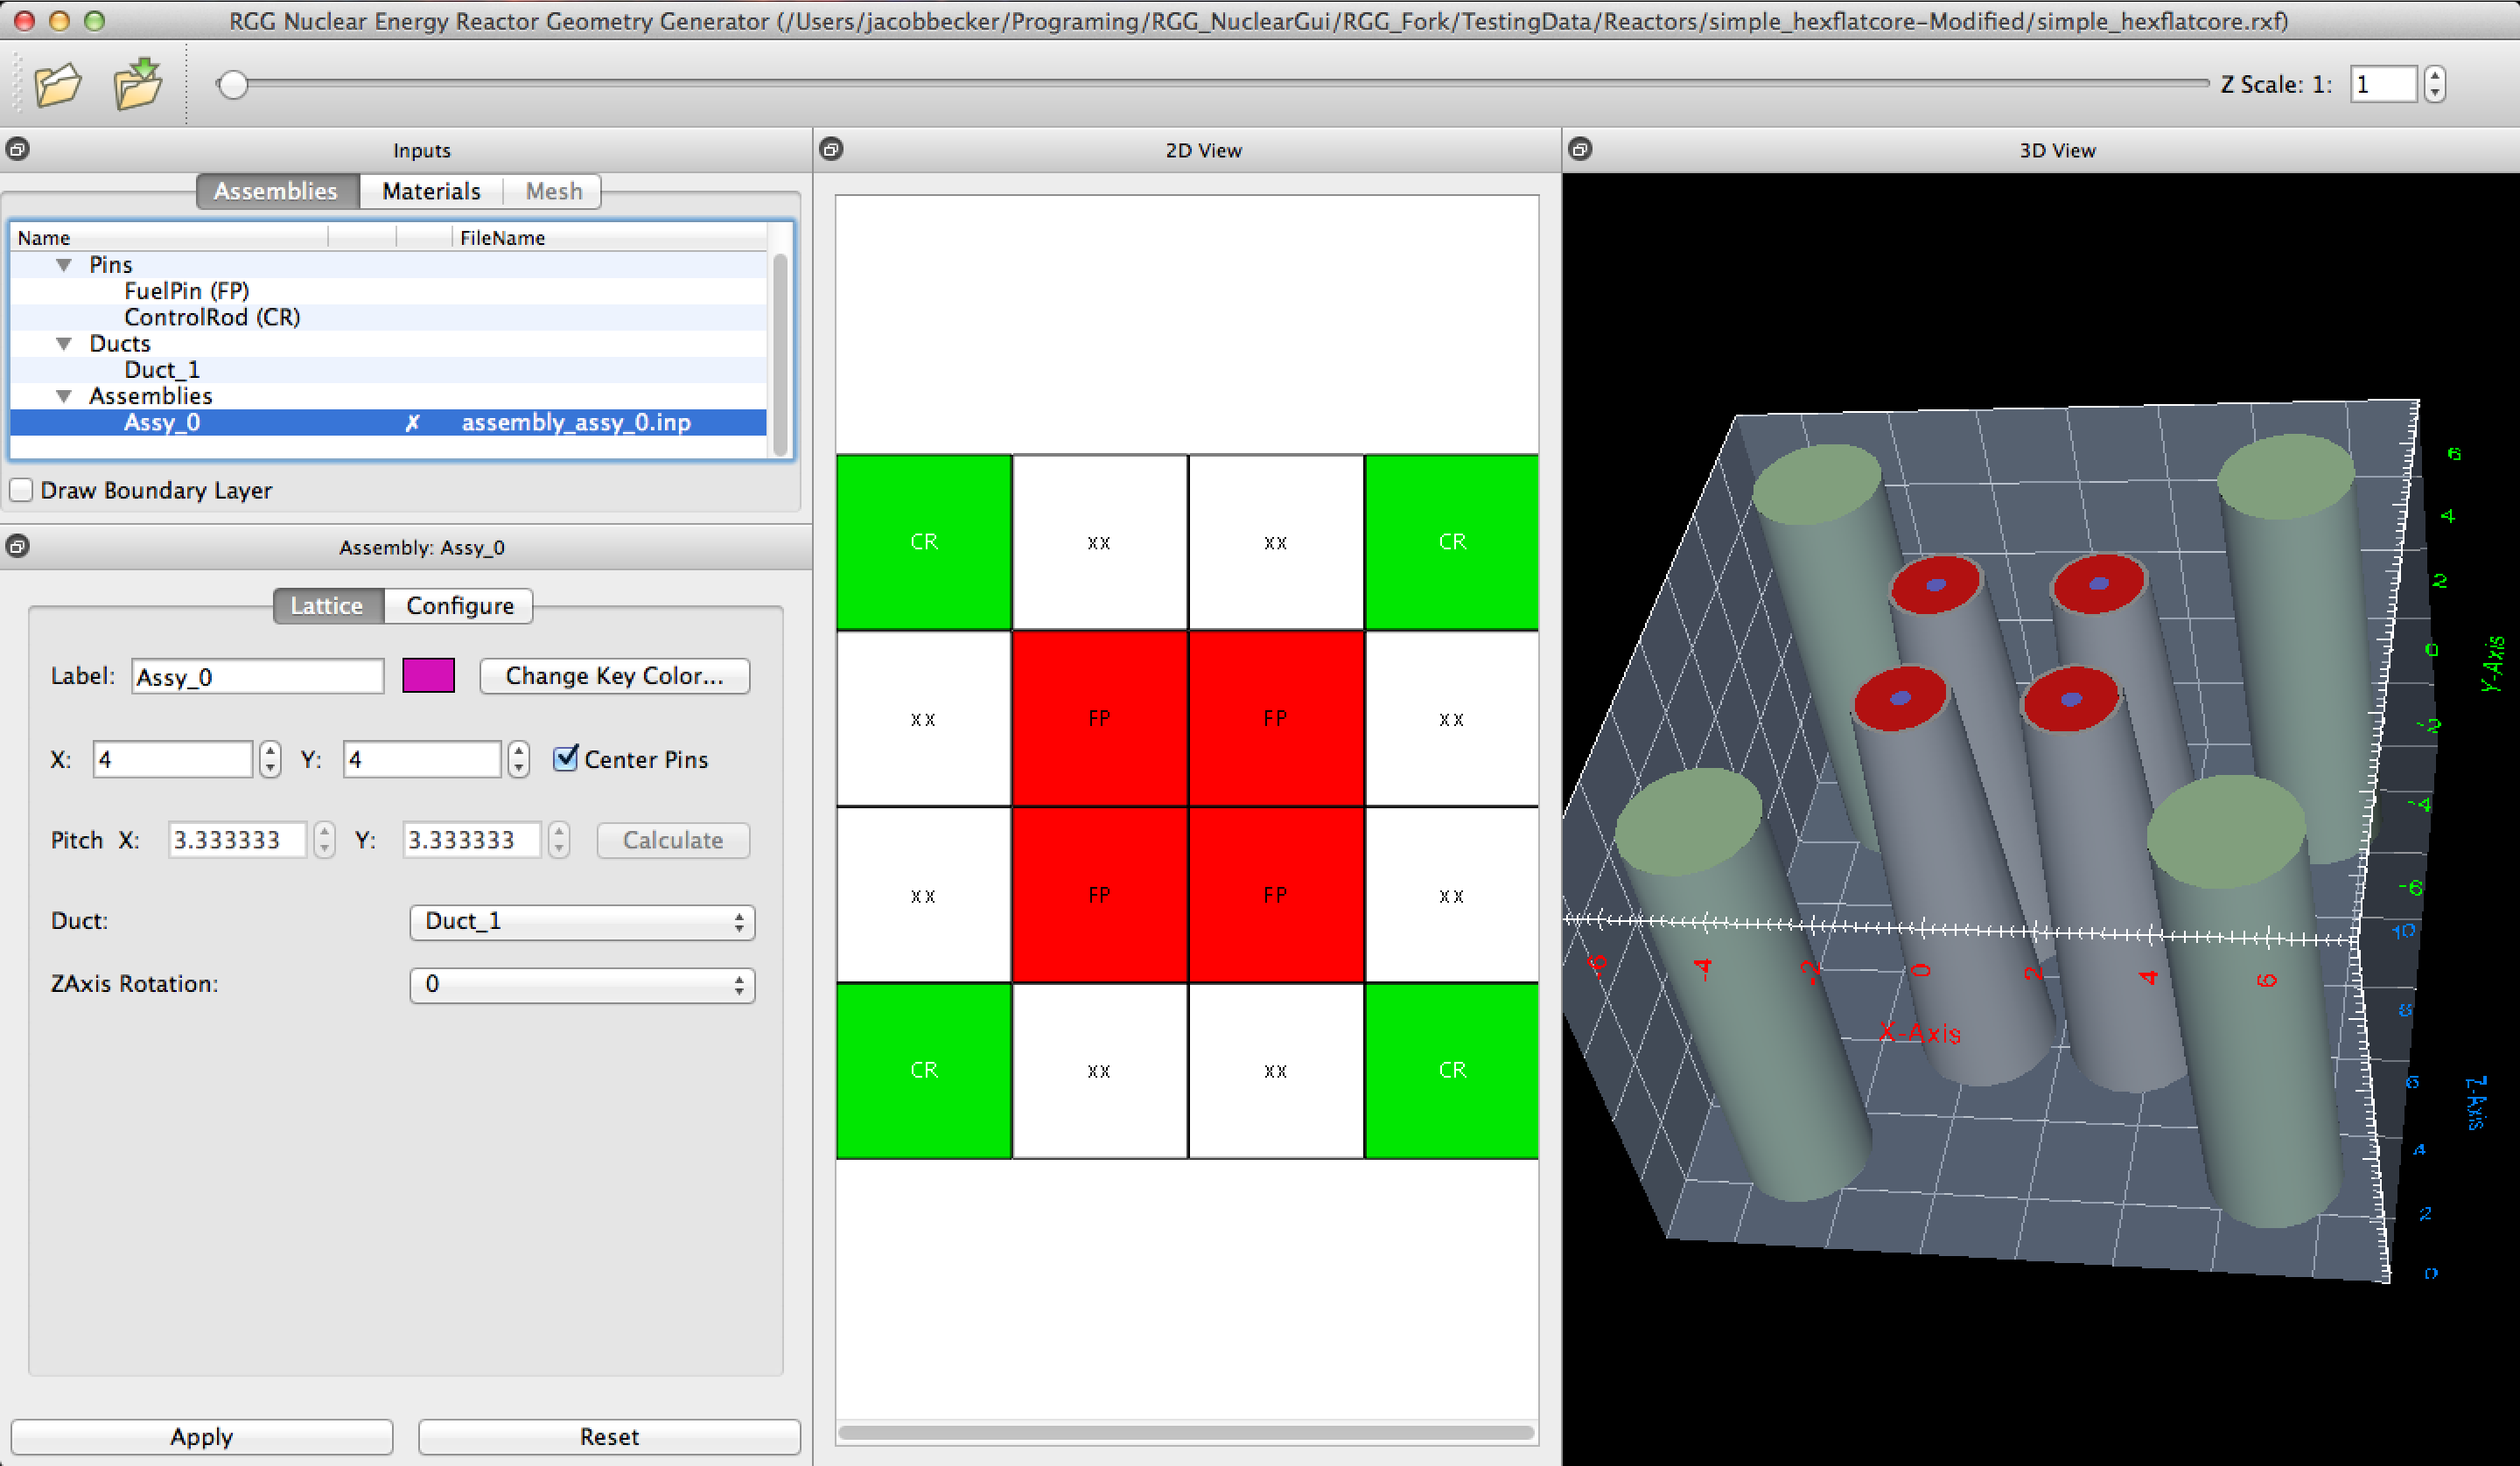
\includegraphics[width=0.60\linewidth]{Images/rect-final-assy1.png}
\caption{Final assembly.}
\label{fig:Rect10}
\end{center}
\end{figure}

